% Figure block + experiment description for the ICASSP submission.
% Figure: figures/avg_width_vs_experts_ETTh1.pdf
% Regenerate with:  python scripts/plot_avg_width_vs_experts.py
%
% Every number below comes from scripts/plot_avg_width_vs_experts.py over seeds
% 4021-4025; coverage from the same records. CP is plotted on the MoE backbone; the
% backbone-matched control (CP on MoG, coverage 0.903, width 1.950) is quoted in the
% text so the CP-MOG gain cannot be read as a backbone artifact.

\begin{figure}[t]
  \centering
  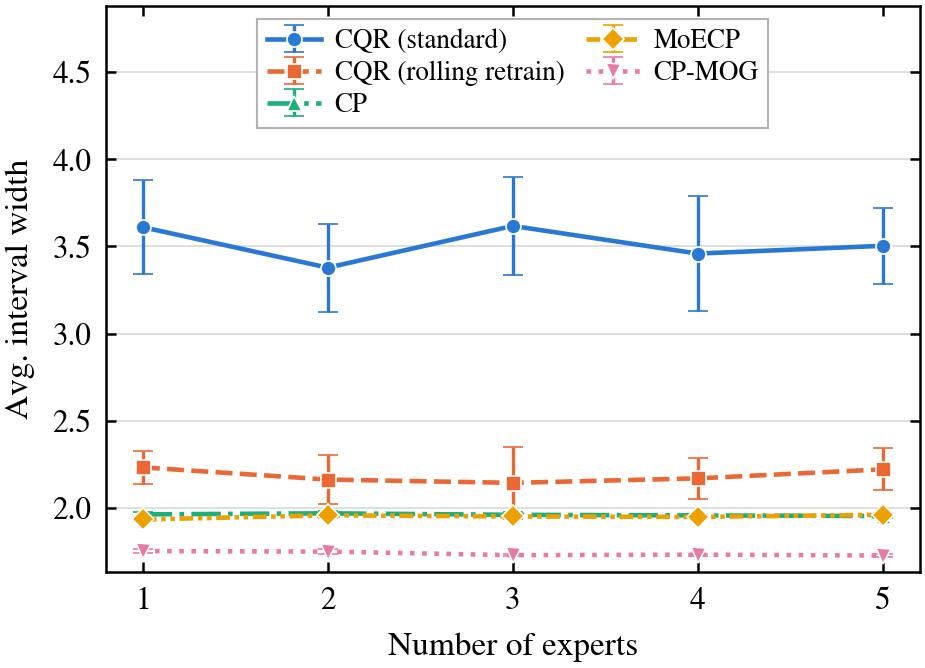
\includegraphics[width=\linewidth]{figures/avg_width_vs_experts_ETTh1.pdf}
  % One-line caption. The coverage numbers, the seed-stability gap and the note
  % about the unresolvable conformal error bars now live in the body paragraph
  % below -- do not drop them, they are what makes the width comparison valid.
  \caption{Average width of the $90\%$ prediction intervals on ETTh1
  (iTransformer, horizon $96$) vs.\ the number of experts; mean $\pm 1$ s.d.\
  over five seeds.}
  \label{fig:width_vs_experts}
\end{figure}

% ---------------------------------------------------------------- body paragraph
\noindent\textbf{Interval width versus mixture size.}
Fig.~\ref{fig:width_vs_experts} compares the five calibration schemes on ETTh1 as
the mixture grows from one to five experts. Because the three conformal variants
all attain the nominal level---empirical coverage $0.903$ (CP), $0.903$ (MoECP)
and $0.900$ (CP-MOG), against a target of $0.900$---their widths are directly
comparable. Under this matched coverage CP-MOG yields the tightest intervals at
every mixture size, averaging $1.738$ against $1.961$ for CP, a $11.4\%$
reduction, while MoECP is essentially indistinguishable from CP ($1.951$ vs.\
$1.961$), with overlapping error bars at four of the five settings. Both CQR
variants are substantially wider ($3.514$ for the standard configuration and
$2.186$ for the rolling-retrain one) and simultaneously under-cover ($0.880$ and
$0.855$), so they are dominated on both axes. They are also markedly less stable
across seeds: the coefficient of variation of the width is $7.7\%$ and $6.2\%$
for the two CQR variants against $0.4$--$0.5\%$ for the conformal ones, a
fifteenfold difference that is why only the CQR error bars are visible in
Fig.~\ref{fig:width_vs_experts}. Since CP-MOG requires the
mixture-density head while CP in the figure is calibrated on the MoE backbone, we
also ran CP on MoG as a backbone-matched control: it reaches coverage $0.903$ at
width $1.950$, so the CP-MOG gain is $10.9\%$ under an identical backbone and is
therefore attributable to the calibration scheme rather than to the density head.
Finally, the number of experts has only a weak influence on width: across
$E\in\{1,\dots,5\}$ the total variation stays within $0.03$ for every conformal
variant---an order of magnitude below the gap between CP-MOG and CP---so the
reduction reported here does not come from mixture capacity.
